\section{Desarrollo}
\subsection{Desv\'ios}

En este experimento realizamos un análisis sobre los desvíos de los vuelos en base al tiempo. Dividimos al año en 12 meses y tomamos el período 2000-2008. Para generar un análisis representativo del comportamiento a escala país decidimos tomar 2 estados con características particulares: deben tener gran cantidad de vuelos de llegada y debía ser uno de cada costa. De este modo tomamos a los estados de California y Florida para realizar el análisis.

\subsubsection{California}

En el siguiente gráfico se puede observar el porcentaje de vuelos desviados en el período mencionado para vuelos con destino a California.

\begin{figure}[h!]
  \begin{center}
	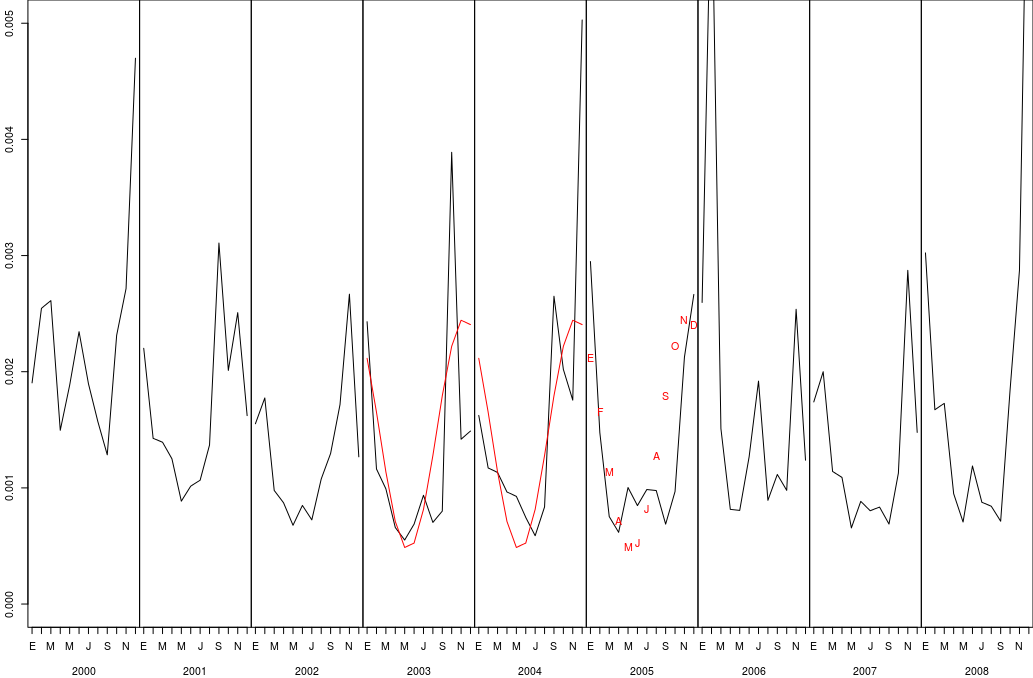
\includegraphics[scale=0.5]{img/plot_CA_2003-2005.png}
	\caption{Diverted arrivals - California}
  \end{center}
\end{figure}

Para aproximar a la función observamos algunas cosas:
\begin{itemize}  
\item Hay cierta periodicidad en la función. Posee picos en los meses correspondientes a las vacaciones de verano del hemisferio norte y descensos en el resto. El período es de 12 meses.
\item Aunque la función tiene picos marcados, su forma se asemeja a la de $sin$ y $cos$.
\end{itemize}

Dados estos indicios nos proponemos encontrar una familia de funciones para aproximar nuestro gráfico usando cuadrados mínimos. Estas funciones serán una combinación de $sin$ y $cos$ con período 12. Las siguientes 2 familias de funciones responden a estas características y aproximan relativamente bien a nuestra función, dados $alpha_i$ correspondientes.


$F_1 = \alpha_1 * abs(sin(\frac{\pi}{12}*x) * cos(\frac{\pi}{6}*x)^2) + \alpha_2$

$F_2 = \alpha_1 * sin(\frac{\pi}{6}*x) + \alpha_2 * cos(\frac{\pi}{6}*x) + \alpha_3$


La primera multiplica al $sin$ y $cos$ y toma el valor absoluto para eliminar los picos negativos. La segunda realiza la suma de los $sin$ y $cos$. No es relevante acá tomar el valor absoluto ya que no hay picos marcados negativos. Luego a ambas funciones le sumamos una constante para que la curva se desplace en dirección vertical. Observamos que sumar una variable lineal no tenía impacto apreciable en la aproximación. 

Luego resolvimos cuadrados mínimos para ambas funciones y calculamos el error cuadrático medio de cada una. Como training tomamos a los años 2003 y 2004 e intentamos predecir 2005.

Los errores cuadráticos medios son: $ECM(F_1) = 0.0003236866$ y $ECM(F_2) = 0.0002451076$, siendo la segunda función una mejor aproximación que la primera. Los valores son pequeños ya que las mediciones son sobre un porcentaje pequeño.

Por lo tanto se puede ver en el gráfico anterior la aproximación que $F_2$ realiza en la muestra, prediciendo cómo será 2005. Se ve que respeta el comportamiento general y aproxima el pico que hay a principio y fin de año.

\subsubsection{Florida}

Realizamos el mismo análisis para los vuelos dirigidos a Florida. Tomamos los mismos 












\begin{figure}[h!]
  \begin{center}
	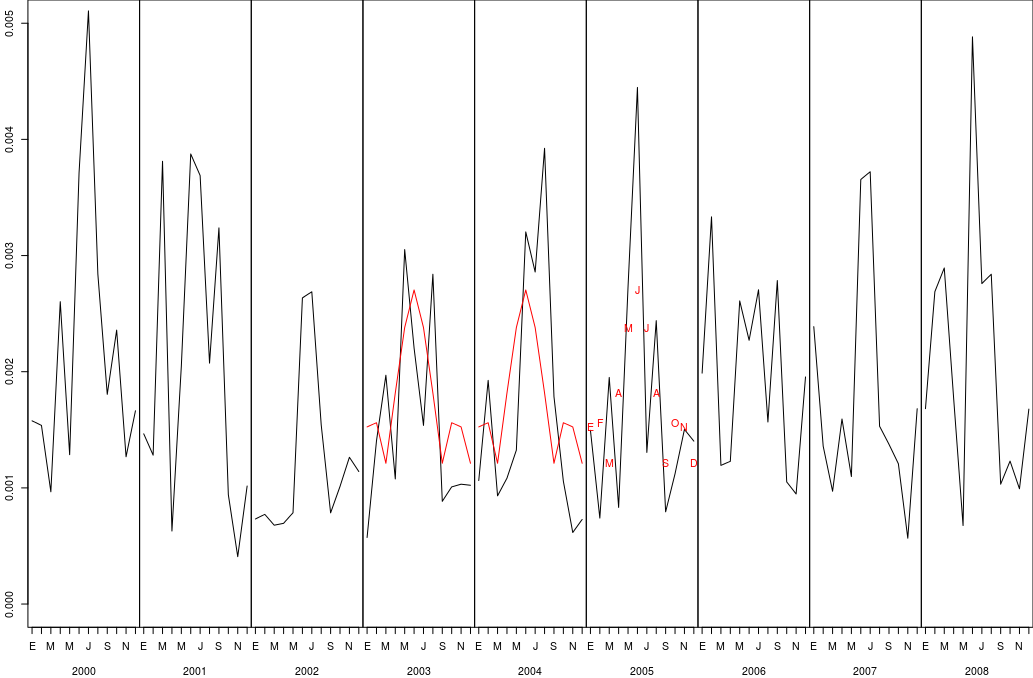
\includegraphics[scale=0.5]{img/plot_FL_2003-2005.png}
	\caption{Diverted arrivals - Florida}
  \end{center}
\end{figure}

$F_1 = \alpha_1 * abs(sin(\frac{\pi}{12}*x) * cos(\frac{\pi}{6}*x)^2) + \alpha_2$

$F_2 = \alpha_1 * sin(\frac{\pi}{6}*x) + \alpha_2 * cos(\frac{\pi}{6}*x) + \alpha_3$

$F_3 = \alpha_1 * abs(sin(\frac{\pi}{12}*x) * cos(\frac{\pi}{6}*x)^2) + \alpha_2 * cos(\frac{\pi}{12}*x - \frac{\pi}{2})^{500} + \alpha_3$
